\section{Probing Algorithm}
\label{sec:ipro_algorithm}

\subsection{Assumptions}
\label{subsec:assumptions}

\subsubsection{Reward}
It defines the objective of any RL-agent. In IPro, the reward targets to ensure the accomplishing of network policies regarding CCO and CUC. Let us consider that the RL-agent chooses an action and increases the probing interval. If IPro does not meet with one or more policies (\textit{e.g.,} policy 1 or policy 2), the RL-agent will learn that it is a wrong action; resulting in a negative reward. Conversely, if IPro meets the policies, the RL-agent will learn that such an increase is a good action; resulting in a positive reward.\\

One of the main RL challenges is to define the reward function. In some cases, the choice of this function is easy because it is implicit in the task. For instance,  in an Atari game, there is a score function that is part of the game itself. In other cases, like in IPro, the choice of such function is complex. The RL-agent has a task objective with multiple criteria, such as keeping CCO and CUC within target values to minimize network performance degradation. In the proposed approach, these criteria are combined in a single scalar-valued reward function using the normal distribution defined by Matignon \textit{et al.} \cite{matignon_2006:improving}, whose heuristic allows defining a multi-objective model useful to consider CCO and CUC (control policies) simultaneously. Therefore, the reward function is defined as follows.

{\setlength{\mathindent}{4cm}
\begin{equation}
    \begin{split}
       R\left ( S_t, A_t \right ) = \beta_c e^{-\frac{d\left ( C\left ( \Theta  \right ), C\left ( \Theta  \right )* \right )^2}{2\sigma_c^2 }} + \beta_u e^{-\frac{d\left ( Us,Us* \right )^2}{2\sigma_u^2 }}
    \end{split}
     \label{equ:reward}
\end{equation}
}

where, $\beta$ adjusts the amplitude of the function and $\sigma$, the standard deviation, specifies the reward gradient influence area. $d$ is the Manhattan distance between the new state $s$ and goal state $s*$. $\Theta$ is the set of active flows in the network. $C\left ( \Theta  \right ) $ and $C\left ( \Theta  \right )*$ are the CCO (cf. equation \ref{equ:load}) used for statistics collection of the set of flows $\Theta$ from the switches in states $s$ and $s*$, respectively. $Us$ and $Us*$ are CUC in states $s$ and $s*$, respectively.\\

\subsubsection{Space of Actions}
The space of actions affects the future state of the network (e.g., the next CCO and CUC), changing the options and opportunities available to the RL-agent at later times. The effects of actions cannot be fully predicted; thus, the RL-agent must monitor the network frequently and react appropriately (i.e., search process). For example, it must watch the probing interval to avoid the breach of policies.

\newlength{\commentWidth}
\setlength{\commentWidth}{7cm}
\newcommand{\atcp}[1]{\tcp*[r]{\makebox[\commentWidth]{#1\hfill}}}
\begin{english_algorithm}
\footnotesize
\SetAlgoLined
\SetKwInOut{Input}{Require}
\SetKwInOut{Output}{Output}

\BlankLine
    \uIf {$action=increase$}{
        Increases the current probing interval}
    \uElseIf{$action=reduce$}{
        Decreases the current probing interval}
    \Else{
        Keeps the current probing interval
      }
\label{alg:actions_algorithm}
\caption{Space of Actions}
\end{english_algorithm}

The RL-agent performs the search process using the action functions (increase, reduce, and keep) in Algorithm 2 to change the probing interval in each iteration and uses the reward function as the guide to the goal state.

\subsubsection{Space of States}
The space of states represents a signal transferring to the agent some sense of ``how the network is'' at a particular time. This space is represented as follows:

{\setlength{\mathindent}{6cm}
\begin{equation}
   % \begin{split}
      S\equiv f \left ( i, l, cpu \right )
%    \end{split}
    \label{equ:states_model}
\end{equation}
}

Each $S_t= \left ( i_t, l_t, cpu_t \right ) \in S$ is characterized by the probing interval $i_t$, CCO $l_t$, and CUC $cpu_t$ in the time $t$. CCO corresponds to the bandwidth consumed by IPro when transmitting and receiving Read-State messages between CP and DP. CUC defines the number of instructions carried out in CP because of IPro tasks (\textit{e.g.}, RL-agent execution, processing of data collection messages). The probing interval indicates how often CP must send Read-State Request messages to retrieve flow statistics from switches in DP.

\subsubsection{Statistics Collection} 
In SDN, the pull-based monitoring is handled by the controller that interacts with the switches via a control channel over TCP. There are two interaction methods \cite{xu_2017:wildcard_requests} \cite{su_2015:cemon}: Per-Flow Collection (PFC) and Per-Switch Collection (PSC). 

\begin{itemize}
    \item In PFC, the controller sends a request to a switch to collect the traffic statistics of one particular flow. This method generates a high CCO when the controller requires to collect statistics of many flows. This overhead is due to the large quantity of Read-State Request messages sent per switch.
    \item In PSC, the controller sends a request to collect the traffic statistics of all flow entries from a switch. This method reduces the number of Read-State Reply messages (Controller$<->$Switch) and, so, reduces CCO and CUC. Nonetheless, if PSC is used excessively with, for instance, a low probing interval, it can cause flow statistics overlapping, high CCO, and high CUC. %In IPro, we use PSC because it allows tuning the probing interval to handle CCO and CUC efficiently.
\end{itemize}{}

This master dissertation focuses on the PSC method because first, PSC generates a smaller amount of Read-State messages that imply lower CCO and CUC. Second, PSC reduces the repeated headers of the flows that involve less redundancy in the collected information \cite{su_2015:cemon}.\\

In IPro, the \textbf{SDN Model} consists of a logically-centralized controller (may be a cluster of distributed controllers \cite{jose_2011:online_measurement} \cite{tahaei_2018:distributed_controller}) and a set of switches. The SDN is modeled by an out-of-band control plane and an undirected graph $G=(V,E)$, where $V=\left \{ v_1,..., v_n \right \}$ is the set of nodes (switches and controllers) and $E=\left \{ e_1,..., e_u \right \}$ is the set of links connecting nodes. This master dissertation assumes that the controller knows the existing active flows in the network, denoted by $\Theta = \left \{ \theta_1, \theta_2, ..., \theta_m \right \} $, with $m=\left | \Theta  \right |$. Thus, it is also reasonable to assume that the controller knows each flow that passes through each switch $v_i$, denoted by $\theta_i$, with $i=1,2,...,m$. Therefore, the active flows number in switch $v_i$ is $\left | \theta_i  \right |$. It is noteworthy that the evaluation of CCO and CUC is critical for any out-of-band CP because, first, the control bandwidth is a limited resource and must be analyzed and optimized. Second, CUC is also a constrained resource that must be used appropriately to avoid the wrong behavior of CP and, so, of the underlying DP.

\subsubsection{Control Channel Overhead} 
CCO is the bandwidth cost used for statistics collection of a set of flows from the switches. In IPro, the controller generates this cost when requests and receives to and from the switches the statistics of a set of flows $\theta_i$. According to \cite{onf_2012:openflow}\cite{su_2015:cemon}, the bandwidth cost caused by $\theta_i$ involves two parts: (\textit{i}) the size of the Read-State Request messages $l_{rq}$ sent to switches; and (\textit{ii}) the size of the Read-State Reply messages  $l_{rp}$ that depends on the number of existing flows $\left | \theta_i  \right |$ in the flow tables. Thus, the bandwidth cost is defined as follows.

{\setlength{\mathindent}{4cm}
\begin{equation}
    C\left ( \Theta  \right ) = l_{rq} \cdot \left | V \right | + l_{rp} \cdot \sum_{i=1}^{\left | V \right |} \left | \theta_i \right |, \forall i \leqslant \left | V \right |
    \label{equ:load}
\end{equation}
}

\subsubsection{CPU Usage of the Controller}
CUC is the number of instructions generated by execution, calculation, and comparison of raw data in IPro. According to \cite{tahaei_2018:distributed_controller}, CUC can be estimated through a constant ($x$) that indicates the number of instructions carried out by CPU to fragment the Read-State Reply messages. Therefore, CUC for analyzing $n$ specific flows from $\Theta$ is modeled as a linear function of $n$.

{\setlength{\mathindent}{3cm}
\begin{equation}
    CPU \cong \left | V \right |* n\left ( ReadStateReply \right ) * x,  \forall n \in \Theta
     \label{equ:load_cpu}
\end{equation}
}
\subsubsection{Monitoring Accuracy} 
MA reflects the difference between the real value of a metric and the measured value by IPro. A smaller difference (error) indicates a higher MA. The error is calculated with the following expression:

{\setlength{\mathindent}{5cm}
\begin{equation}
    \begin{split}
        \%error = \frac{\left | v_{C}-v_{R} \right |}{v_{R}}*100
    \end{split}
     \label{equ:percent-error}
\end{equation}
}
where, $v_{C}$ is the measured value of the metric being monitored and $v_{R}$ is the real value (or reference). Therefore, MA is as follows:
{\setlength{\mathindent}{5cm}
\begin{equation}
    \begin{split}
        MA = 100\% - \%error
    \end{split}
     \label{equ:ma}
\end{equation}
}

\subsection{Functioning}
\label{subsec:assumptions}

Algorithm 3 presents the probing interval optimization procedure carried out by IPro. The algorithm inputs are the learning factor $\alpha$, the discount factor $\gamma$ (\textit{cf.} Equation~\ref{equ:q_function}), and the exploration method $\varepsilon$ (cf. Equation~\ref{equ:e-greedy}). The output is the most-rewarding probing interval according to the current network status.\\

The probing algorithm has two considerations: \textit{i}) it assumes a null initial condition of the $Q(\mathcal{S},\mathcal{A})$ before the first update occurs (line 1); and \textit{ii}) it starts its execution from a random state that represents the initial values of probing interval, CCO, and CUC (line 3). After these considerations, the probing interval optimization process begins (line 4). In this process, the RL-agent discovers the reward structure and determines the most-rewarding probing interval by interacting with the network. The proposed algorithm performs the following steps in each iteration (lines 5 to 13):

\newlength{\commentWidth}
\setlength{\commentWidth}{7cm}
\newcommand{\atcp}[1]{\tcp*[r]{\makebox[\commentWidth]{#1\hfill}}}
\begin{english_algorithm}
\footnotesize
\SetAlgoLined
\SetKwInOut{Input}{Require}
\SetKwInOut{Output}{Output}

\Input{
    \\
    %States $\mathcal{S} = \{1, \dots, n_s\}$ \\
    %Actions $\mathcal{A} = \{1, \dots, n_a\},\qquad A: \mathcal{S} \Rightarrow \mathcal{A}$ \\
    %Actions $\mathcal{A} = \{up, down, equal\},\qquad A: \mathcal{S} \Rightarrow \mathcal{A}$ \\
    %Reward function $R: \mathcal{S} \times \mathcal{A} \rightarrow \mathbb{R}$ \\
    Exploration parameter  $\varepsilon$ \\
    %Transition function ($\epsilon$) $T: \mathcal{S} \times \mathcal{A} \rightarrow \mathcal{S}$ \\
    Discount factor $\gamma$ \\
    Learning factor $\alpha$ \\
    %Reward function $R: (S,A) \rightarrow R $
}
\KwResult{A probing interval}

%Initialize $Current Bandwidth$ $CB$\;
%Calculate current traffic according to Control and Monitoring messages $CM$ \;
%\If{$ CM > CB * 0.8 $}{
\BlankLine
Initialize $Q:$ $Q(\mathcal{S},\mathcal{A})=0, \forall s \in \mathcal{S}, \forall a \in \mathcal{A}$
\BlankLine
    \While{not reached stopping criterion}{
      Start in state $S_{t} \in \mathcal{S}$\;
      %Choose A from $S_{t}$ using policy derived from $\underset{\rm A}{\rm max} Q_{t}(S_{t},A)$\;
        \While{$S_{t}$ is not terminal}{
            Select $A_{t}$ from $S_{t}$ using policy derived from Q using $\varepsilon$-greedy exploration method\;
            %Calculate $\pi$ according to Q \;
            %Exploration strategy (e.g. $\pi(x) \gets \argmax_{a} Q(s, a)$)\;
            $A_{t} \gets \pi(S_{t})$ \tcp*[h]{Execute probing action}\;
            Modify the probing interval according to the action $A_{t}$\;
            $S_{t+1} \gets T(S_{t}, A_{t})$ \tcp*[h]{Receive the new state}\;
            $R_{t+1} \gets R(S_{t}, A_{t})$ \tcp*[h]{Calculate reward}\;
            $Q_{t+1}(S_t,A_t) \leftarrow & (1-\alpha) \cdot Q_{t}(S_t,A_t) +
             &\alpha \cdot \left [R_{t+1} + \gamma \cdot \underset{\rm A}{\rm max} Q_{t}(S_{t+1},A) \right]$\tcp*[h]{Update Q-function}\;
            %Modify the probing interval according to the action $A_{t}$\;
            Send the probing interval modified to Data Repository\;
            $S_{t} \gets S_{t+1}$ \tcp*[h]{Move to the new state}\;
            $t \gets t+1$  \tcp*[h]{Increment and set the number of steps taken}\;
        }
    }
%}
%\Return $Q$
%\caption{$Q$-learning: Learn Function $Q: \mathcal{S} \times \mathcal{A} \rightarrow \mathbb{R}$}
\label{alg:ipro_algorithm}
\caption{Probing Interval Optimization}
\end{english_algorithm}
%\bigskip % add 12pt space in-between

\begin{itemize}
    \item The RL-agent selects a probing action $A_{t}= \{up, down, equal\}$ from the Q-function using the $\varepsilon$-greedy exploration method that modifies the probing interval (line 7). The possible actions are to increase ($up$), reduce ($down$), or keep ($equal$) the probing interval.
    \item The RL-agent executes the probing action selected in the previous step (line 6). Since this execution affects the network behavior, the network falls in a new state. MP determines the new state by Equation~\ref{equ:states_model}, where CCO and CUC are determined using Equation~\ref{equ:load} and Equation~\ref{equ:load_cpu}, respectively. The value of the probing interval is obtained in the step 1. Subsequently, MP sends this new state to the RL-agent.
    \item The RL-agent receives the new network state from MP (line 8). 
    \item The RL-agent takes such a state to calculate the reward (line 9). In particular, the reward is computed by Equation~\ref{equ:reward}.
    \item Based on the learning factor, discount factor, initial considerations, reward, and new network state, the RL-agent tunes the values of the Q-function according to Equation~\ref{equ:q_function} (line 10).
    \item The RL-agent sends the probing interval to \textit{Data Repository} (line 11).
    \item The RL-agent moves to the new state (line 12) and moves on to the next iteration $t+1$ (line 13).
\end{itemize}

The probing interval optimization process is repeated until the agent perceives that the policy does not change. At this moment, the agent gets the most-rewarding probing interval that keeps CCO and CUC within target values aiming at minimizing network performance degradation caused by the monitoring tasks.

\subsection{Computational Complexity}
\label{subsec:computational-complexity}

IPro determines its optimal policy by finding an Optimal Value Function. The Optimal Value Function of a policy is the expected infinite discounted reward that will be gained, at each state, by executing that policy.  This value can be computed by the Equation~\ref{equ:total-reward}, where $Q_{t}(S_{t},A) = E\left ( \sum_{t=0}^{\infty} \gamma^{t}R_{t} \right )$. Once the IPro RL-agent knows the value of each state under the current policy, it considers whether the value could be improved by changing the first action taken. If the value can be improved, the RL-agent changes the policy to take the new action whenever it is in that situation. This step guarantees an improvement in the performance of the policy strictly. When no enhancements are possible, then the policy is optimal.\\

Since IPro operates by successive approximations of an Optimal Value Function, its computational complexity, per iteration, is quadratic in the number of states ($S$) and linear in the number of actions ($A$): ($O\left ( \left | A \right |\left |  S\right |^{2} \right )$). Furthermore, the number of iterations required to reach the Optimal Value Function is polynomial in the number of states and the magnitude of the highest reward if the discount factor is held constant. In the worst case, the number of iterations grows polynomially in $\frac{1}{1-\gamma }$. Thus, the IPro RL-agent convergence rate slows considerably as the discount factor nearby 1.

\subsection{IPro Interactions}
\label{subsec:sequence-diagram}

IPro uses RL to optimize the probing interval regarding CCO and CUC. For higher compression of how the IPro architecture elements interact at run time, the analysis is divided into two general parts: statistics collection process and probing interval optimization process.

\subsubsection{Statistics Collection Process}
\label{subsec:statistics-collection-process}

\begin{figure}[h!]
    \centering
    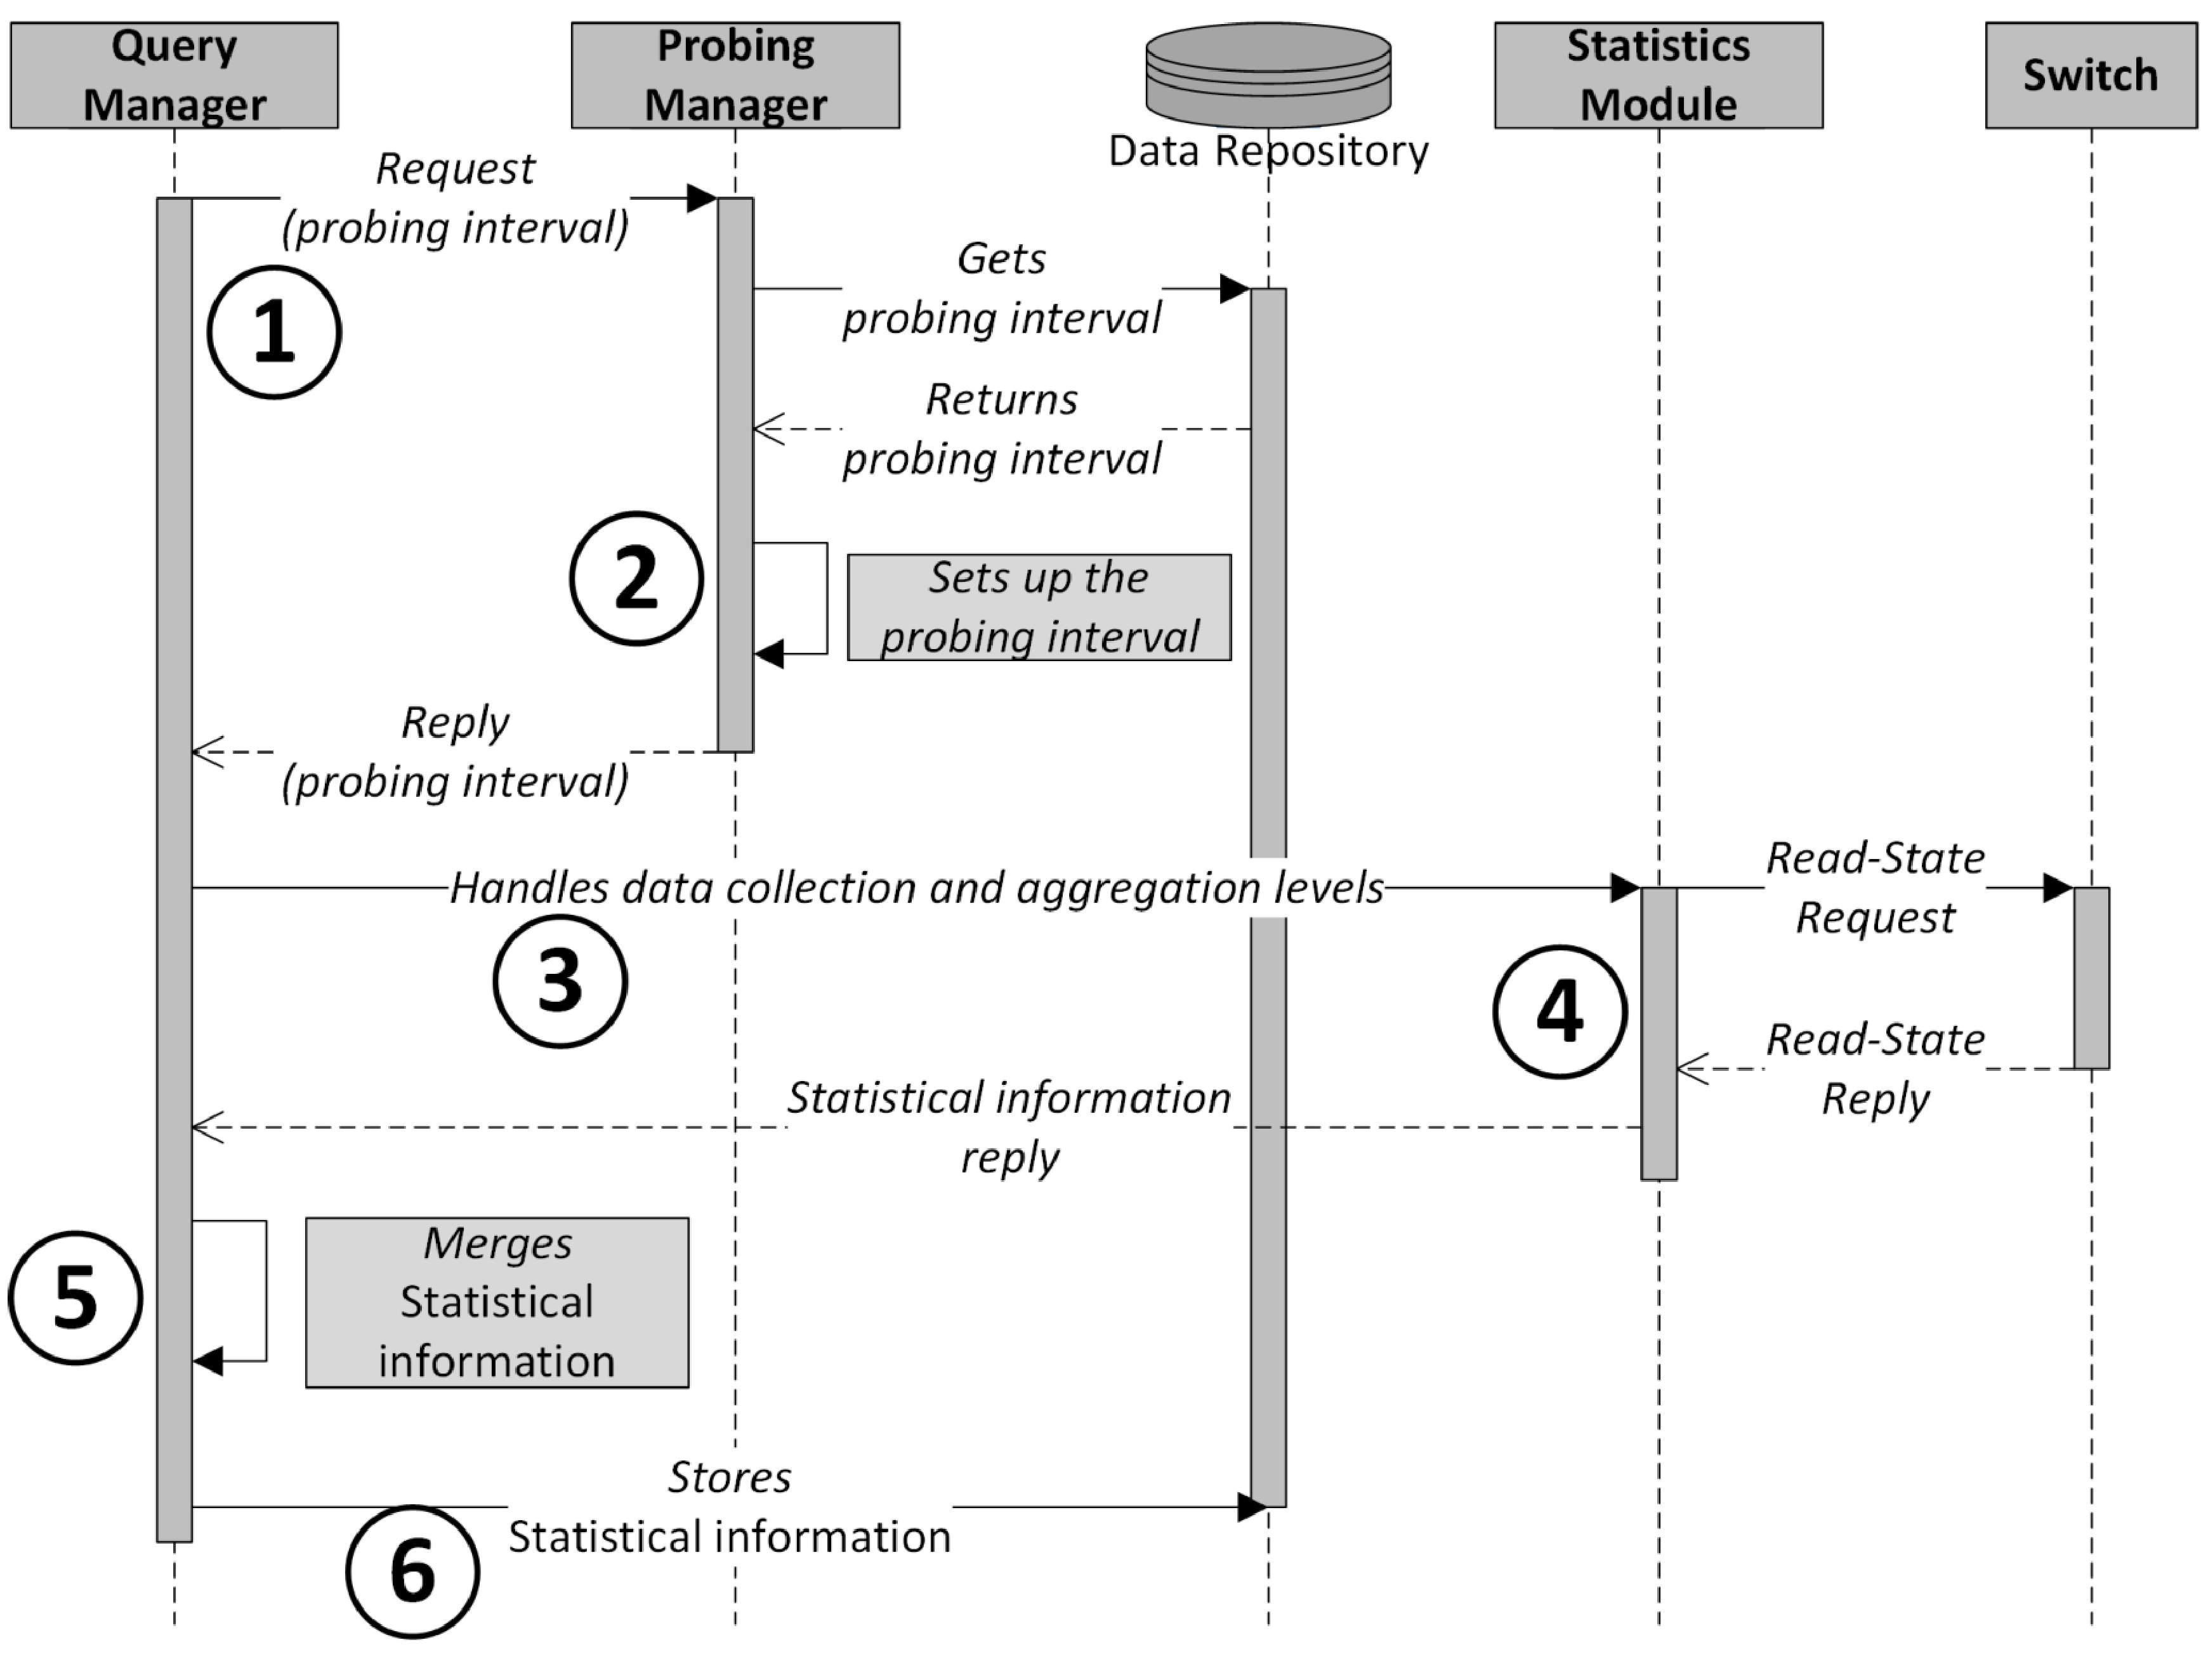
\includegraphics[width=0.90\columnwidth]{figures/Figure5-IPro-Sequence-diagram-cp}
    \caption{Sequence diagram of statistics collection process}
    \label{fig:sequence-diagram-cp}
\end{figure}

Figure~\ref{fig:sequence-diagram-cp} depicts how the elements of CP and DP interact in the statistics collection process. 

\begin{enumerate}[label=\protect\circled{\arabic*}]
    \item Query Manager requests Probing Manager to set up the probing interval to handle the data collection.
    \item Probing Manager consults the data repository to know the probing interval and sets up it how the current interval.
    \item Query Manager handles the data collection based on the current probing interval and the desired aggregation levels (\textit{e.g.}, byte, packet, flow).
    \item Statistics Module collects statistical information from the switch at the current probing interval using Read-State messages (request and reply). After this data collection, Query Manager merges \circled{5} and stores \circled{6} the statistical information into the Data Repository. Thus, this information can be used ulteriorly by upper-layer applications.
\end{enumerate}

It is important to highlight that the collection process affects network behavior; the network falls in a new state.

\subsubsection{Probing Interval Optimization Process}
\label{subsec:probing-interval-optimization-ptocess}

\begin{figure}[h!]
    \centering
    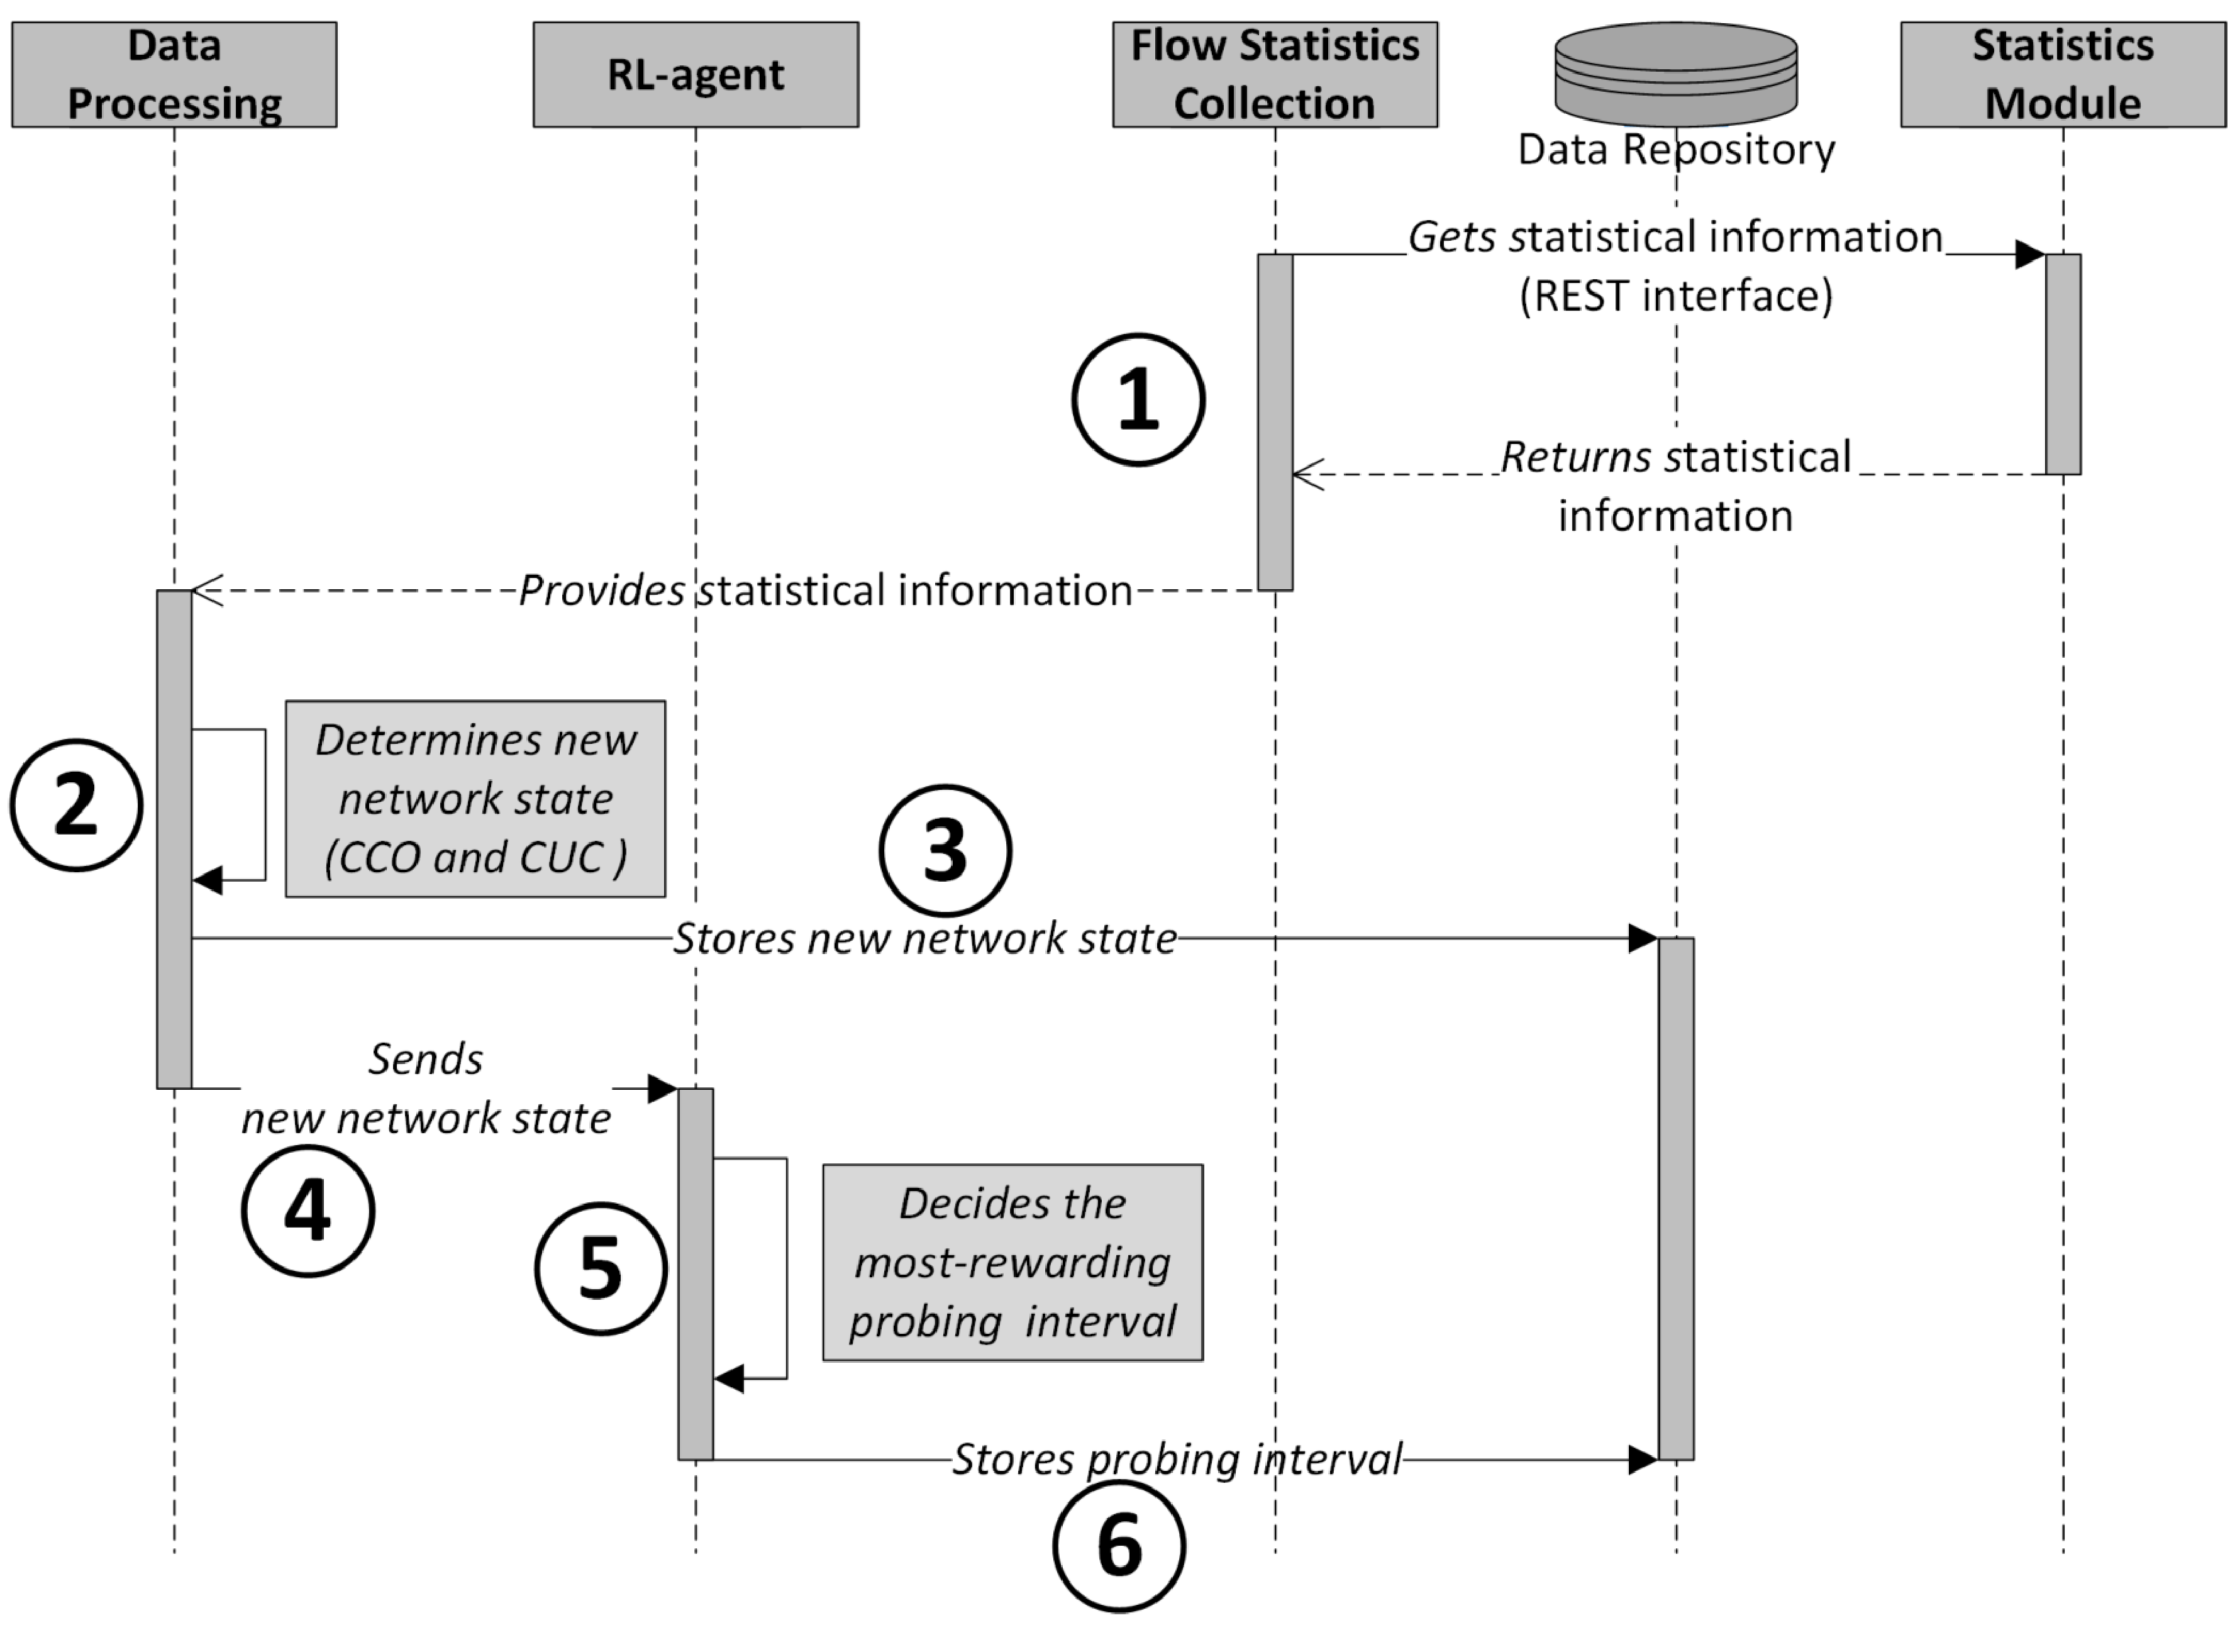
\includegraphics[width=0.90\columnwidth]{figures/Figure6-IPro-Sequence-diagram-mp}
    \caption{Sequence diagram of probing interval optimization process}
    \label{fig:sequence-diagram-mp}
\end{figure}

Figure~\ref{fig:sequence-diagram-mp} depicts how the elements of MP and KP interact in the probing interval optimization process.

\begin{enumerate}[label=\protect\circled{\arabic*}]
    \item Flow Statistics Collection extracts the statistical information from the Statistics Module located at CP and provides this information to Data Processing.
    \item Data Processing processes and organizes the information retrieved by Flow Statistics Collection to determine and such a new state by analyzing CCO and CUC.
    \item Data Processing stores the new state.
    \item Data Processing sends the new state to RL-agent located at KP.
    \item The RL-agent takes such a state to calculate the reward. Based on the reward, the RL-agent decides the most-rewarding probing interval intended to minimize CCO and CUC.
    \item The RL-agent stores this new probing interval to Data Repository. Probing Manager applies this interval that affects the network behavior again (\textit{i.e.}, initiates Statistics Collection Process). This process continues until the network administrator decides to stop IPro.
\end{enumerate}
